\documentclass[aspectratio=169,11pt,hyperref={colorlinks=true}]{beamer}
\usetheme{boxes}
\setbeamertemplate{navigation symbols}{}
\definecolor{openstack}{RGB}{149,0,4}
\setbeamercolor{titlelike}{fg=openstack}
\setbeamercolor{structure}{fg=openstack}
\hypersetup{colorlinks,urlcolor=openstack}
\setbeamertemplate{footline}[frame number]
% Inserting graphics
\usepackage{graphicx}
% Side-by-side figures, etc
\usepackage{subfigure}
% Code snippits
\usepackage{listings}
% Color stuff
\usepackage{color}
\usepackage{amsmath}
\usepackage{tikz}
\newcommand\RBox[1]{%
  \tikz\node[draw,rounded corners,align=center,] {#1};%
}
\usepackage{hyperref}
%\usecolortheme{buzz}
%\usecolortheme{wolverine}
%\usetheme{Boadilla}
\usepackage[T1]{fontenc}

\definecolor{mygreen}{rgb}{0,0.6,0}
\definecolor{mygray}{rgb}{0.5,0.5,0.5}
\definecolor{mymauve}{rgb}{0.58,0,0.82}

\lstset{%
  backgroundcolor=\color{white},   % choose the background color; you must add \usepackage{color} or \usepackage{xcolor}
  breakatwhitespace=false,         % sets if automatic breaks should only happen at whitespace
  breaklines=true,                 % sets automatic line breaking
  captionpos=b,                    % sets the caption-position to bottom
  commentstyle=\color{openstack},  % comment style
  extendedchars=true,              % lets you use non-ASCII characters; for 8-bits encodings only, does not work with UTF-8
  keepspaces=true,                 % keeps spaces in text, useful for keeping indentation of code (possibly needs columns=flexible)
  keywordstyle=\color{blue},       % keyword style
%  otherkeywords={*,...},           % if you want to add more keywords to the set
  numbersep=5pt,                   % how far the line-numbers are from the code
  numberstyle=\tiny\color{mygray}, % the style that is used for the line-numbers
  rulecolor=\color{black},         % if not set, the frame-color may be changed on line-breaks within not-black text (e.g. comments (green here))
  showspaces=false,                % show spaces everywhere adding particular underscores; it overrides 'showstringspaces'
  showstringspaces=false,          % underline spaces within strings only
  showtabs=false,                  % show tabs within strings adding particular underscores
  stringstyle=\color{openstack},   % string literal style
}

\setbeamerfont{caption}{series=\normalfont,size=\fontsize{6}{8}}
\setbeamertemplate{caption}{\raggedright\insertcaption\par}

\setlength{\abovecaptionskip}{0pt}
\setlength{\floatsep}{0pt}

\author[Matthew Treinish]{%
    \texorpdfstring{%
        \centering
        Matthew Treinish\\
        \href{mailto:mtreinish@kortar.org}{mtreinish@kortar.org}\\
        \texttt{mtreinish on Freenode}
   }
   {Matthew Treinish}
}
\date{May 11, 2017}

\title[Dirty Clouds Done Dirt Cheap
\hspace{2em}\insertframenumber/\inserttotalframenumber]{Dirty Clouds Done Dirt Cheap}

\begin{document}

{%
\setbeamertemplate{background canvas}{
\includegraphics[width=\paperwidth,height=\paperheight]{background_title.png}}
\setbeamertemplate{footline}{}
\begin{frame}[noframenumbering]
    \setbeamercolor{titlelike}{fg=white}
    \setbeamercolor{structure}{fg=white}
    \setbeamercolor{normal text}{fg=white}
    \hypersetup{colorlinks,urlcolor=white}
    \setbeamercolor{author}{fg=white}
    \setbeamercolor{date}{fg=white}
    \setbeamercolor{background}{bg=openstack}
    \titlepage{}
    \centering
    \href{https://github.com/mtreinish/dirty-clouds-done-dirt-cheap}{https://github.com/mtreinish/dirty-clouds-done-dirt-cheap}
\end{frame}
}

\section{Building a Cloud}
\begin{frame}
\frametitle{Building a Cloud}
\centering
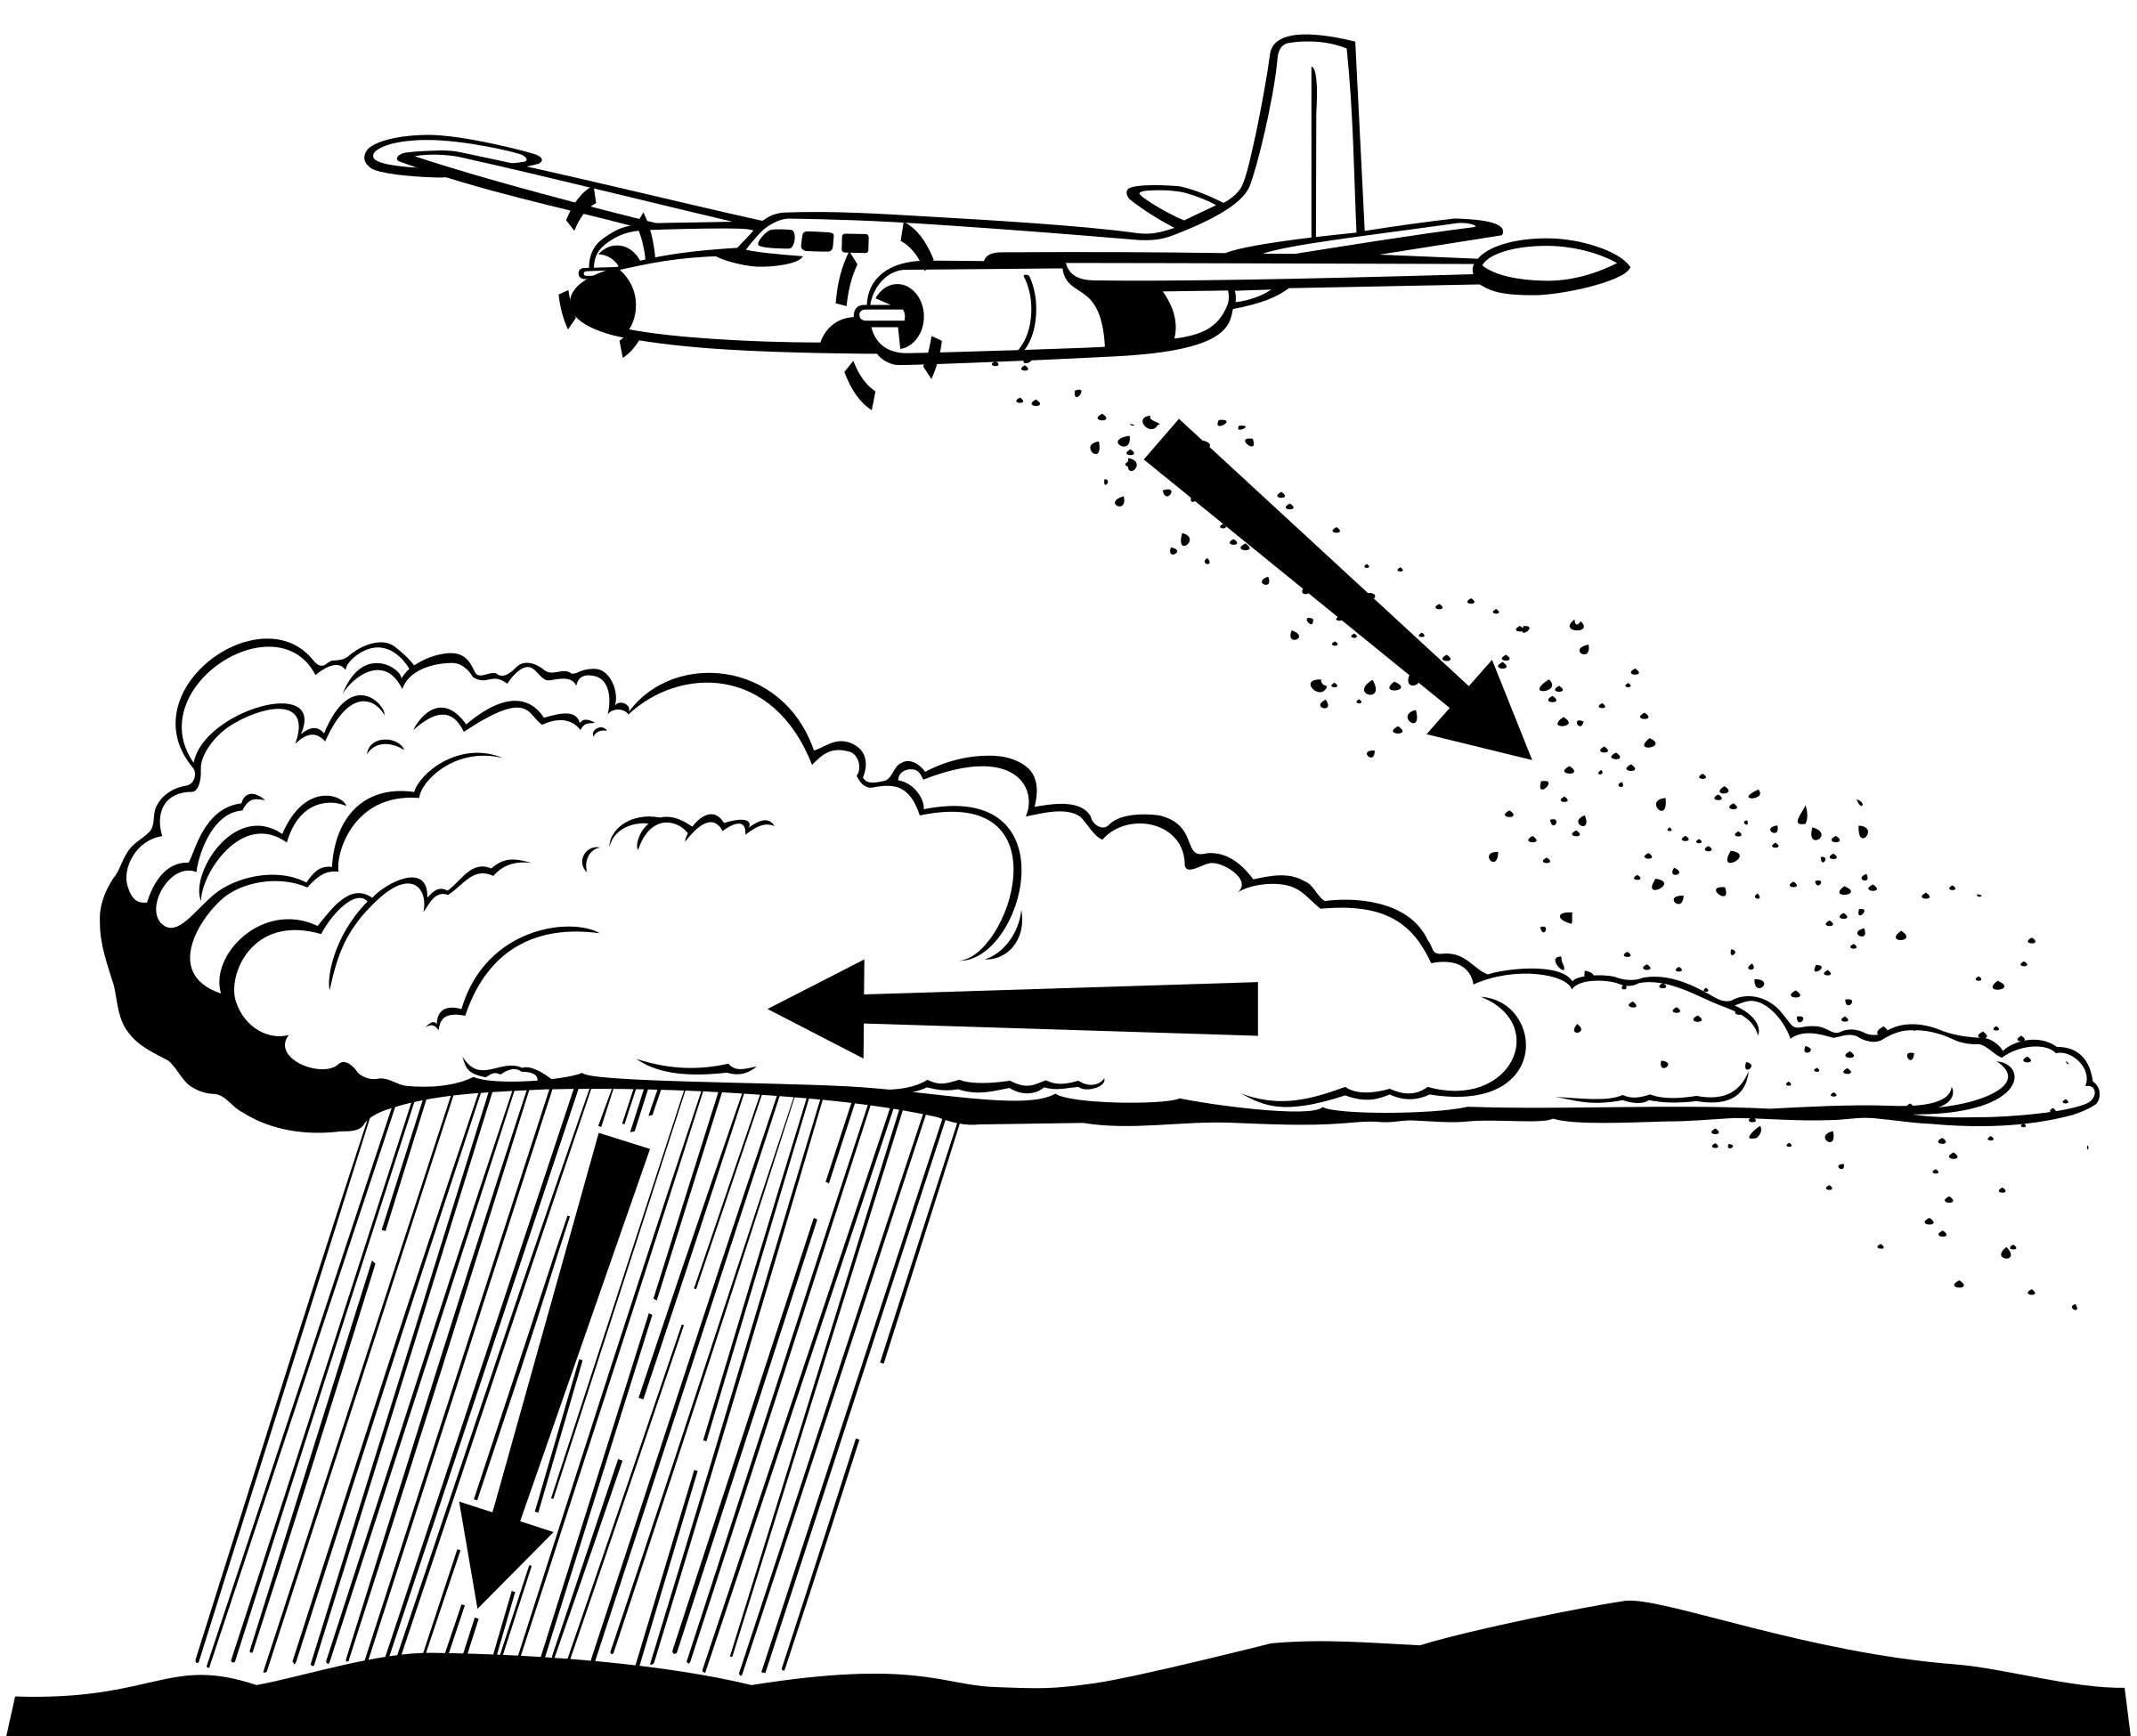
\includegraphics[width=.775\textwidth]{cloud_seeding.png}
\end{frame}

\begin{frame}
\frametitle{Scope of the Project}
    \begin{itemize}
        \item Pretend to be a sysadmin with no prior OpenStack knowledge
        \item Try to rely only on install docs and google searches
        \item \$1500 USD Budget
        \item Build a basic compute cloud:
        \begin{itemize}
            \item Keystone
            \item Glance
            \item Nova
            \item Neutron
        \end{itemize}
        \item Install Ocata from tarballs
        \item No automation or pre-existing install scripts
    \end{itemize}
\end{frame}

\begin{frame}
\frametitle{Buying Hardware}
    \begin{itemize}
        \item Maximize core count per USD
        \item Second priority is amount of RAM per core
        \item Machines don't need to be fast (that costs money!)
    \end{itemize}
\end{frame}

\begin{frame}
    
\includegraphics[width=\textwidth]{EBay_logo.png}
\end{frame}

\begin{frame}
    \frametitle{The Servers}
    \begin{tabular}{ l c r }
        \hline
        Model &	PowerEdge R610 \\
        \hline
        Processor &	2x Intel Xeon E5540 \\
        \hline
        Memory Installed & 32GB Total Memory; 8 x 4 GB DDR3 \\
        \hline
        Hard Drives & 2x 146GB 10K SAS Hard Drive \\
        \hline
        RAID Controller & Dell PowerEdge R610 Perc 6i \\
        \hline
        Ethernet & 2x Dual Port Embedded Broadcom NetXtreme ll 5709c \\
        \hline
        Return Policy/Warranty & 60 days Money Back Or Exchange \\
        \hline
    \end{tabular}
    \\
    \begin{center}
        \Huge{\textbf{\$215 Each!!}}
    \end{center}
\end{frame}

\begin{frame}
    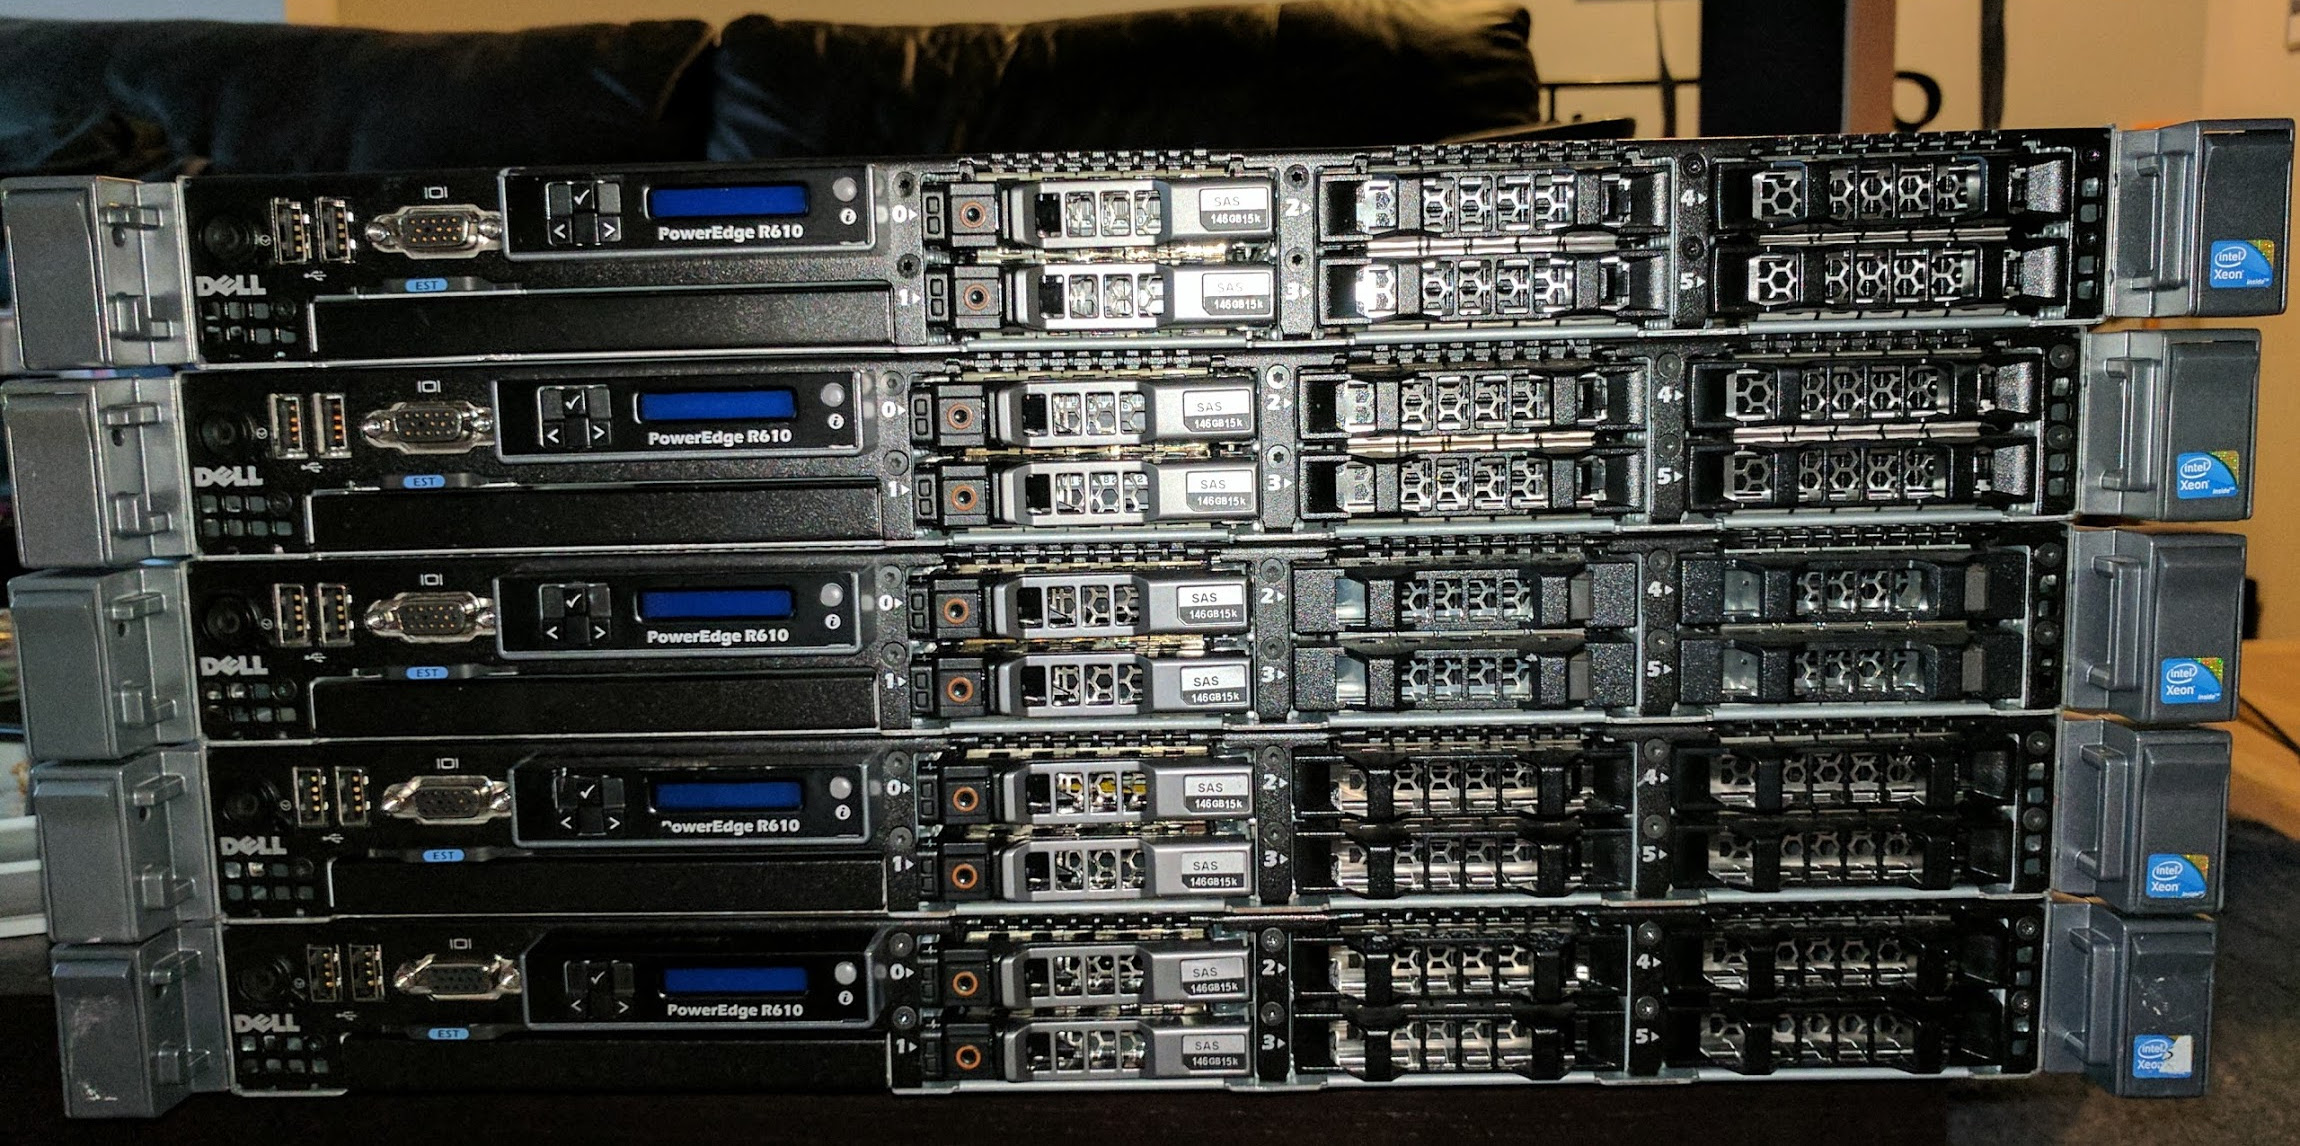
\includegraphics[width=\textwidth]{servers_delivered.jpg}  
\end{frame}

\begin{frame}
    \frametitle{Quirks with the servers}
    \begin{itemize}
        \item Super stripped down:
            \begin{itemize}
                \item No management interface
                \item No redundant power supply
            \end{itemize}
        \item 4x8GB of RAM not 8x4GB
        \item Memory installed in wrong slots
        \item Dead RAID controller battery
        \item Came with 15k RPM hard drives not 10k RPM
        \item Came pre-installed with Windows Server 2012 (and default password Apple123)
        \item At full fan speed \textbf{>70 dB}
    \end{itemize}
\end{frame}

\begin{frame}
\frametitle{Assembling the Cloud}
    \begin{itemize}
        \item Need something to hold the servers
        \item Traditional racks are too much money (even used)
    \end{itemize}
\end{frame}

\begin{frame}
    \frametitle{LackRack}
    \href{https://wiki.eth0.nl/index.php/LackRack}{https://wiki.eth0.nl/index.php/LackRack}
    \begin{columns}[T]
        \begin{column}{.48\textwidth}
            \begin{itemize}
                \item Use a LACK side table from Ikea
                \item 19 inch width between legs
                \item Can fit 8U
                \item Lots of color choices
                \item \$9.99 USD
            \end{itemize}
        \end{column}
        \begin{column}{.48\textwidth}
            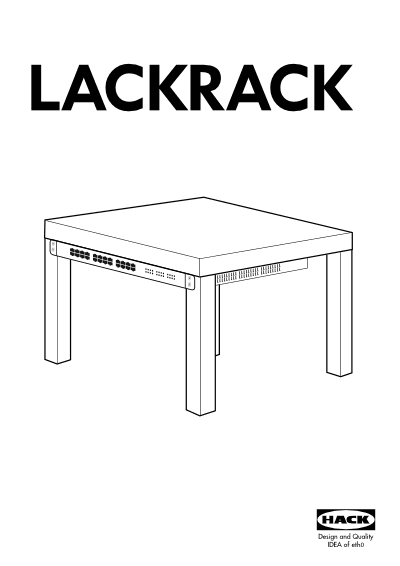
\includegraphics[width=\textwidth]{lackrack_cover.png}
        \end{column}
    \end{columns}
\end{frame}

\begin{frame}
    \centering
    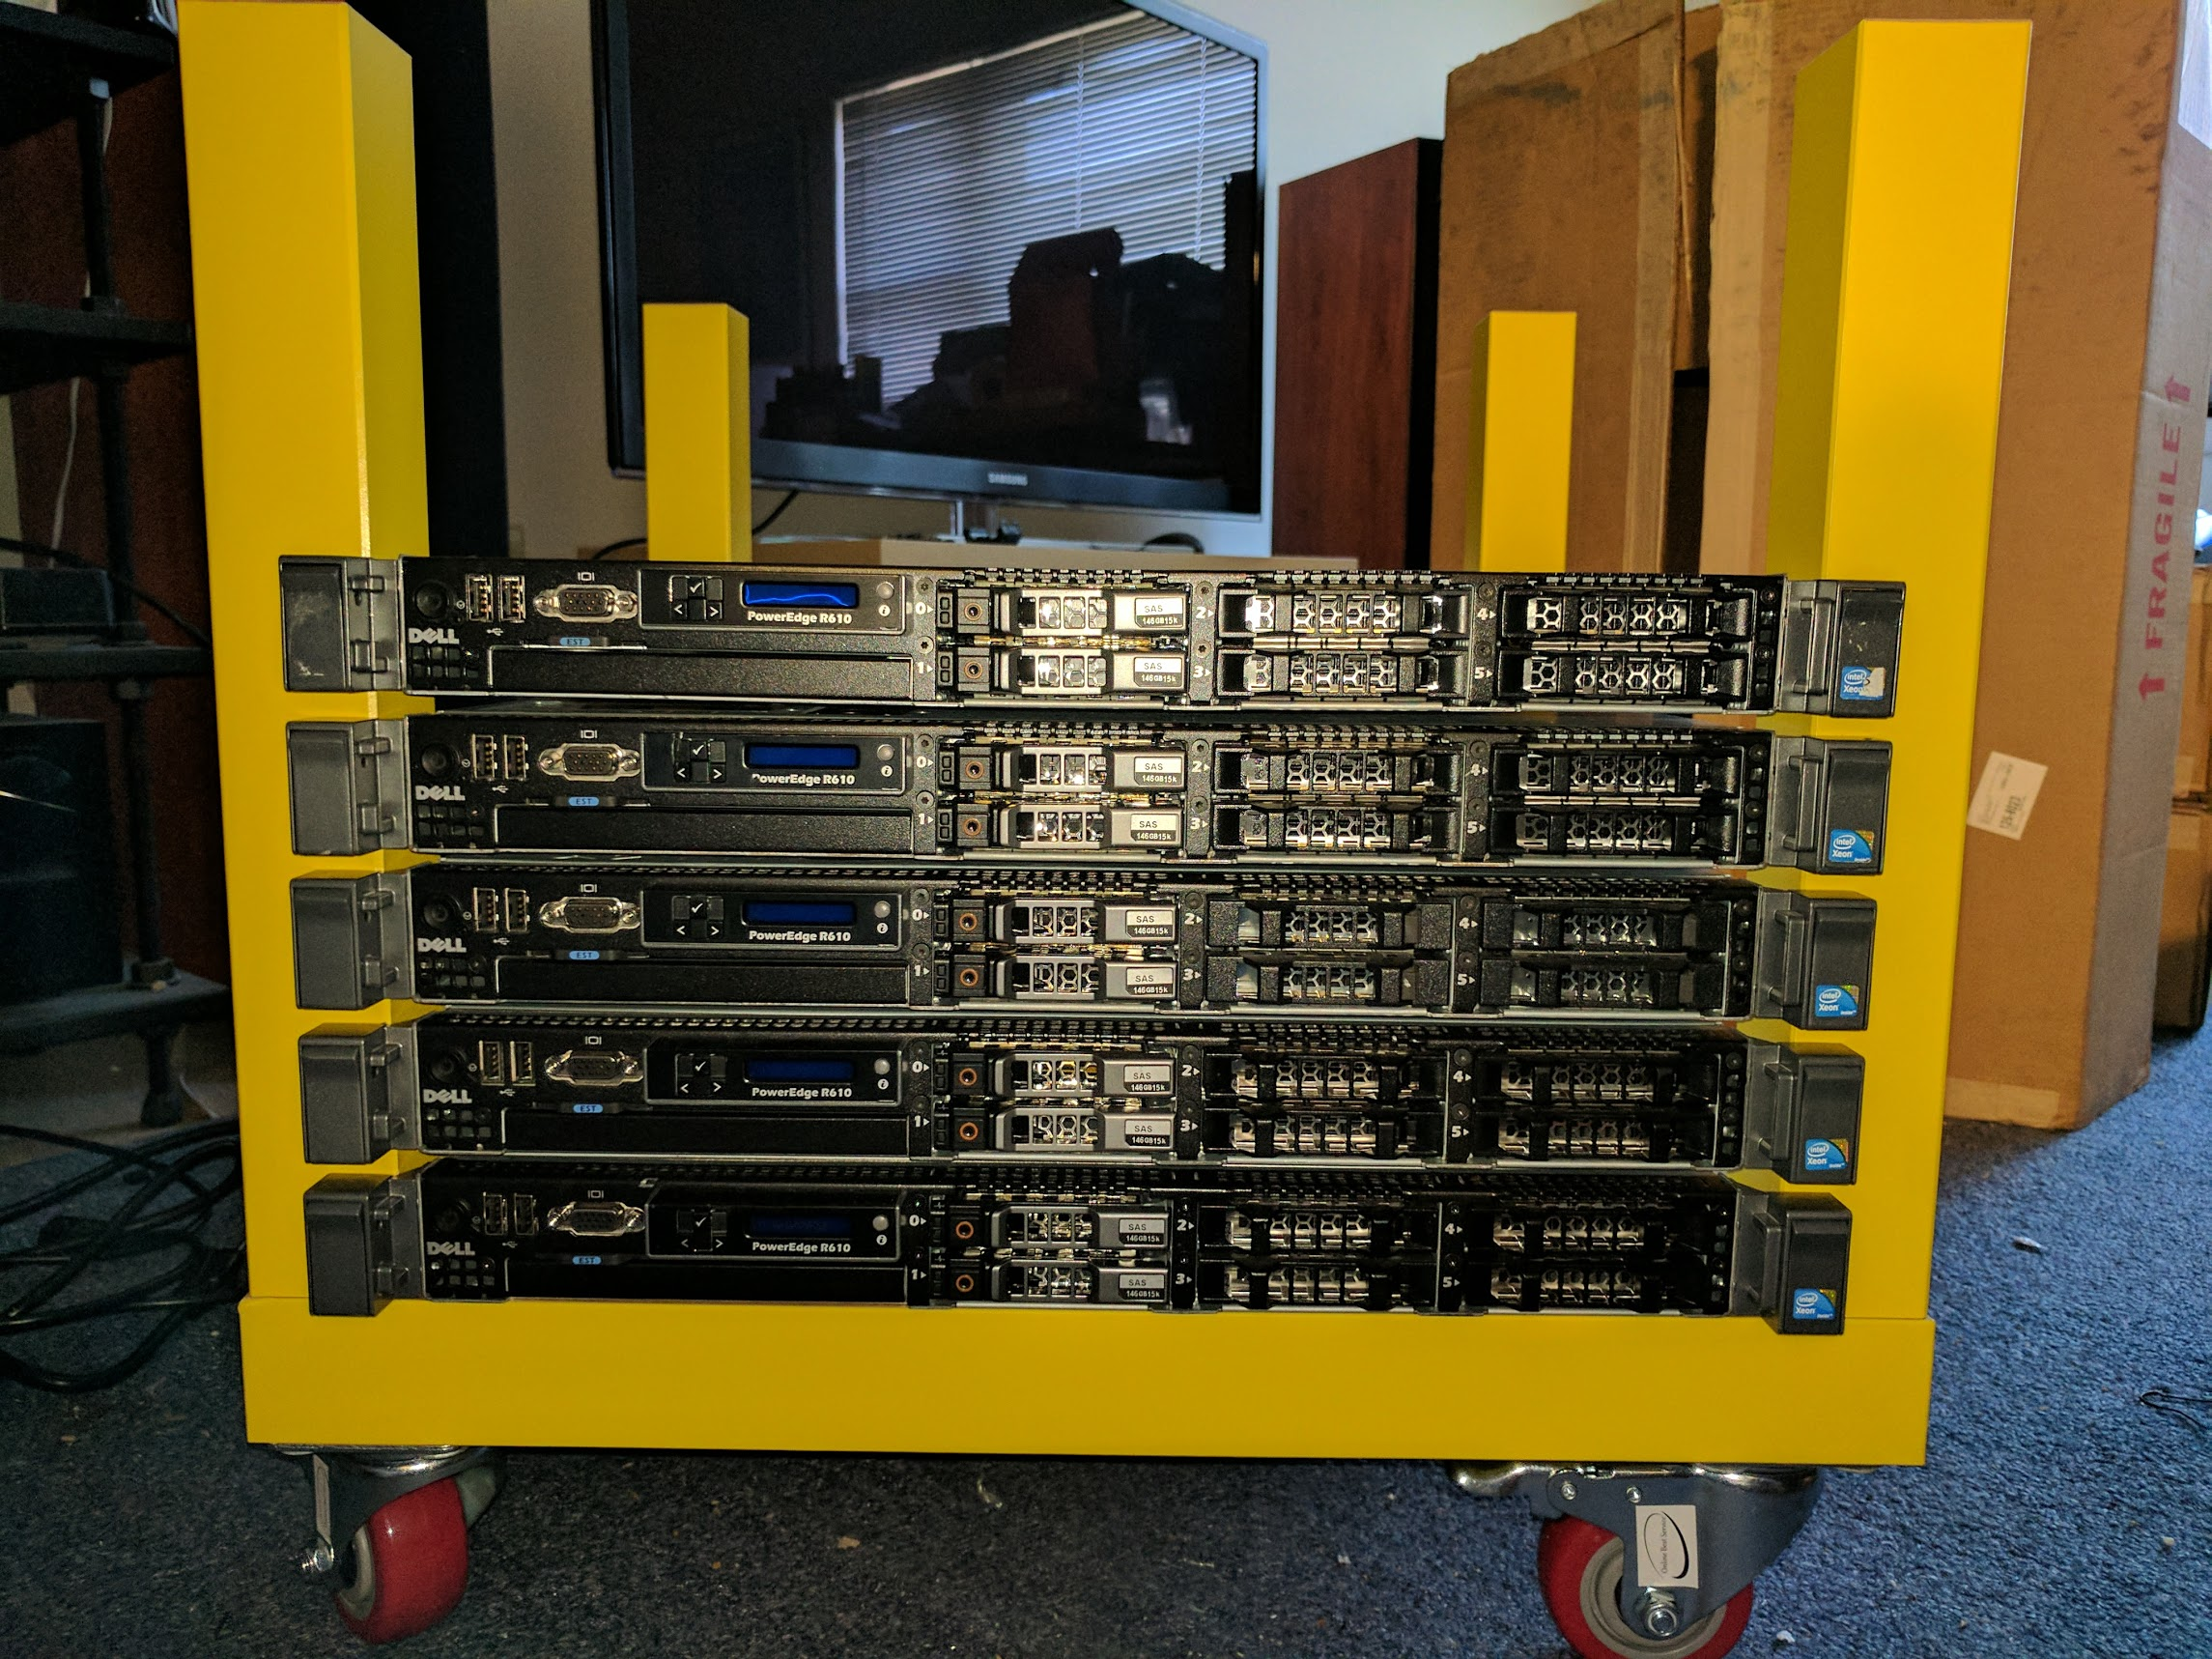
\includegraphics[width=.75\textwidth]{lack_rack.jpg}
\end{frame}

\begin{frame}
    \centering
    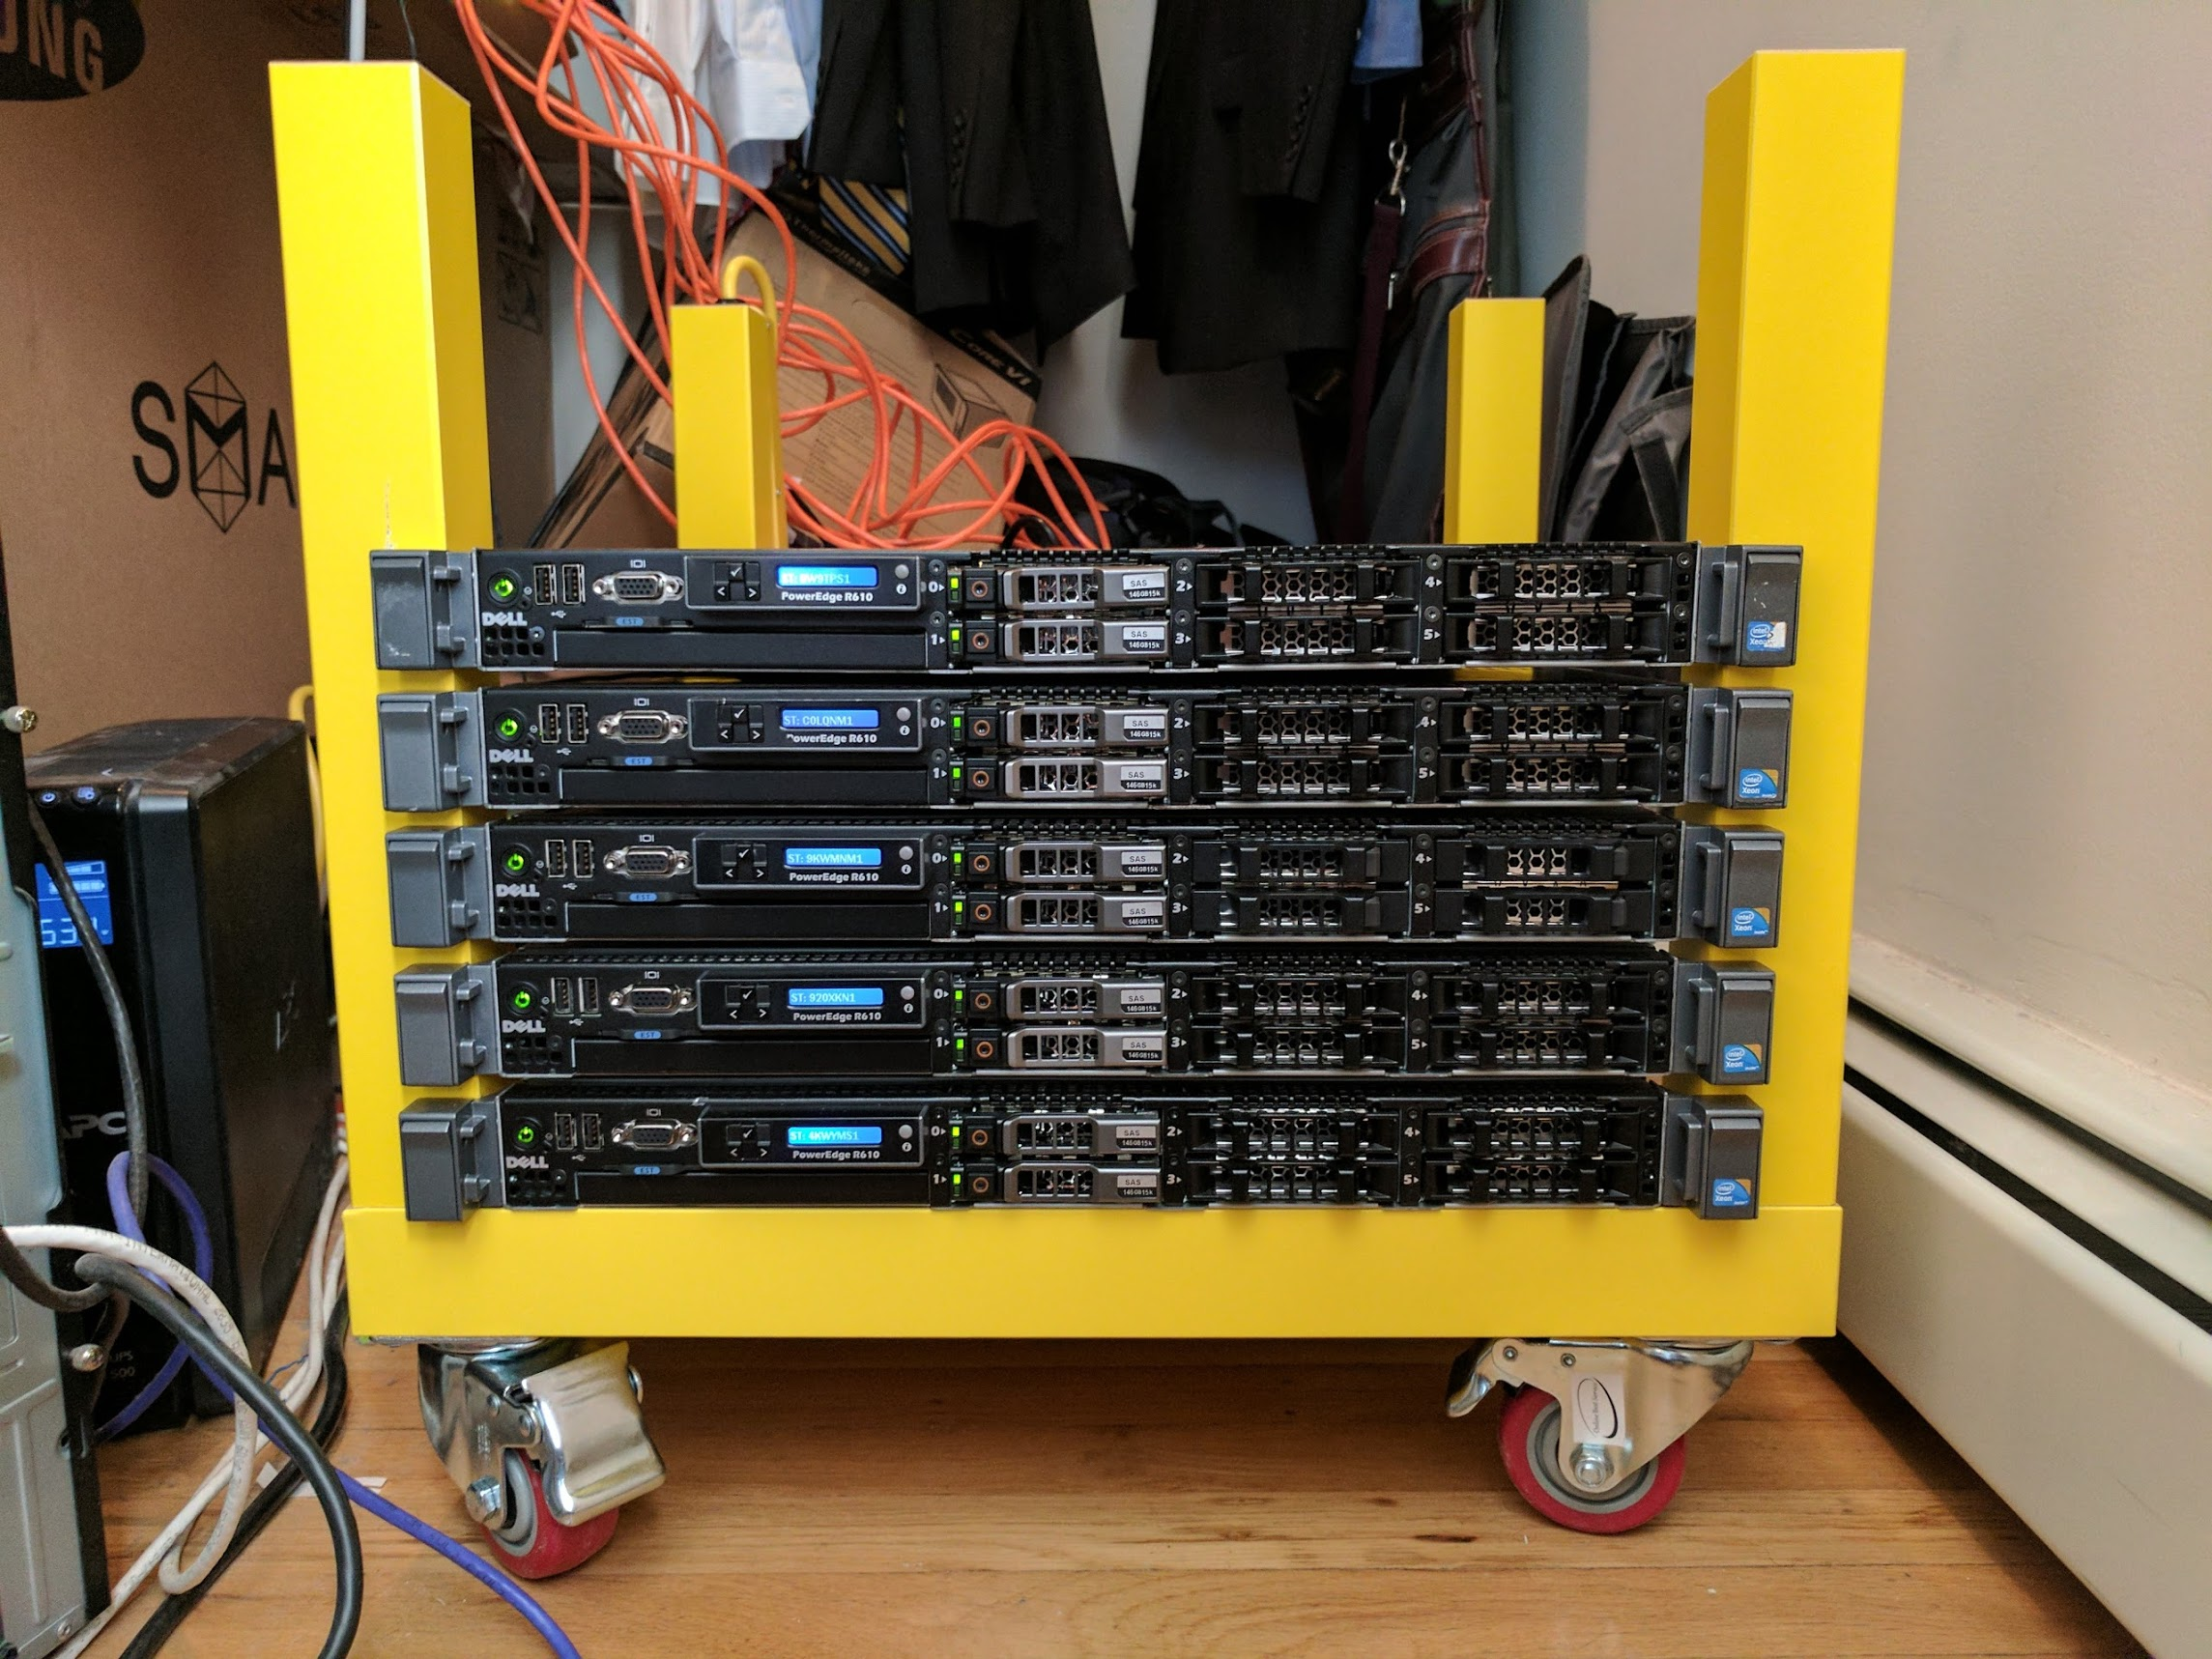
\includegraphics[width=.9\textwidth]{data_closet.jpg}
\end{frame}

\section{Installing the OS}
\begin{frame}
    \frametitle{Installing the Operating System}
    \begin{itemize}
        \item Installed Ubuntu 16.04 LTS server
        \item Nothing special, stick with base packages
    \end{itemize}
\end{frame}

\section{Installing OpenStack}
\begin{frame}
    \frametitle{Installing OpenStack}
    \centering
    \includegraphics[width=.8\textwidth]{service-split.eps}
\end{frame}
\begin{frame}
    \frametitle{Installing OpenStack Services}
    \begin{enumerate}
        \item Download service tarball
        \item Create service users
        \item Install binary requirements
        \item Create service dirs in /etc and /var/lib
        \item Copy etc/ from tarball into /etc/\$Service
        \item pip install the tarball
        \item Follow install guide on project configuration and setup
    \end{enumerate}
\end{frame}

\subsection{Installing the Controller}
\subsubsection{Keystone}
\begin{frame}
    \frametitle{Setting Up Keystone}
    \begin{columns}[T]
        \begin{column}{.48\textwidth}
            \begin{itemize}
                \item 2 config options
                \item Install guide doesn't have instructions on
                    apache wsgi app setup
                \item Google search found: \href{https://docs.openstack.org/developer/keystone/apache-httpd.html}{https://docs.openstack.org/developer/keystone/apache-httpd.html}
            \end{itemize}
        \end{column}
        \begin{column}{.48\textwidth}
            
\includegraphics[width=\textwidth]{mascots/keystone.eps}
        \end{column}
    \end{columns}
\end{frame}

\begin{frame}
    \frametitle{Python Requirements aren't fun}
    \lstinputlisting[basicstyle=\tiny,language=python]{notes/keystone-start-failure-cut}
\end{frame}

\subsubsection{Glance}
\begin{frame}
    \frametitle{Setting up Glance}
    \begin{columns}[T]
        \begin{column}{.48\textwidth}
            \begin{itemize}
                \item Straightforward configuration:
                    \begin{itemize}
                        \item Auth
                        \item Image Directories
                        \item Database
                    \end{itemize}
            \end{itemize}
        \end{column}
        \begin{column}{.48\textwidth}
            
\includegraphics[width=\textwidth]{mascots/glance.eps}
        \end{column}
    \end{columns}
\end{frame}

\begin{frame}
    \frametitle{Don't forget to create glance store directory}
    \lstinputlisting[basicstyle=\tiny,language=python]{notes/glance-store-error-cut}
\end{frame}

\subsubsection{Nova}
\begin{frame}
    \frametitle{Setting up Nova}
    \begin{columns}[T]
        \begin{column}{.48\textwidth}
            \begin{itemize}
                \item Database migrations are slower, took about 3mins
                \item Don't forget the placement API, no docs on apache setup
                \item novnc is problematic from source
            \end{itemize}
        \end{column}
        \begin{column}{.48\textwidth}
            
\includegraphics[width=\textwidth]{mascots/nova.eps}
        \end{column}
    \end{columns}
\end{frame}

\begin{frame}
    \frametitle{Requirements still aren't fun}
    \lstinputlisting[basicstyle=\tiny,language=python]{notes/nova-requirements-error-cut}
\end{frame}

\begin{frame}
    \frametitle{Don't forget your sudoers file}
    \lstinputlisting[basicstyle=\tiny,language=python]{notes/nova-sudo-error-cut}
\end{frame}

\begin{frame}
    \frametitle{Don't forget to create state directories}
    \lstinputlisting[basicstyle=\tiny,language=python]{notes/nova-statedir-error-cut}
\end{frame}

\subsubsection{Neutron}
\begin{frame}
    \frametitle{Networking Configuration}
    \centering
    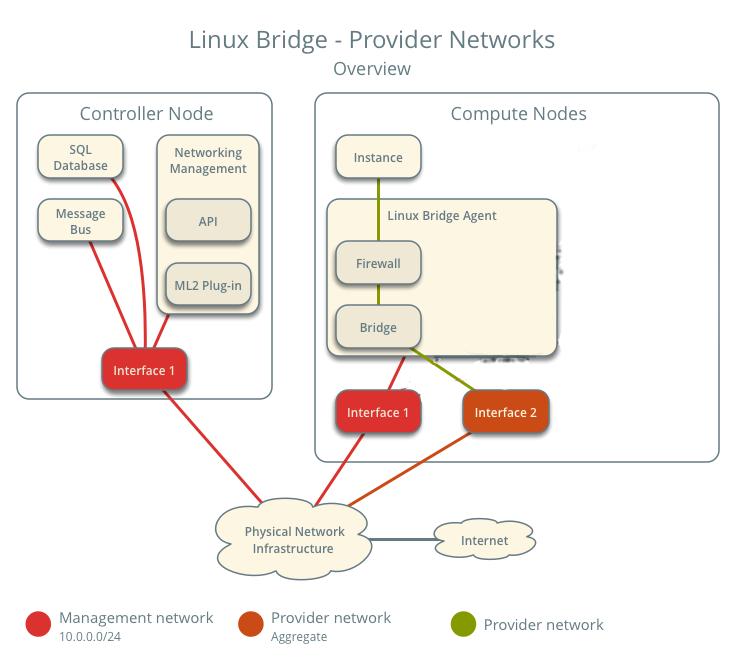
\includegraphics[width=.7\textwidth]{network-topology.png}
\end{frame}

\begin{frame}
    \frametitle{Setting Up Neutron}
    \begin{columns}[T]
        \begin{column}{.48\textwidth}
            \begin{itemize}
                \item Too many configuration files
                \item Blindly copying pasting from install guide
                \item Rootwrap and sudo configuration are not documented
                \item First time I had to look at packages and/or devstack
            \end{itemize}
        \end{column}
        \begin{column}{.48\textwidth}
            
\includegraphics[width=\textwidth]{mascots/neutron.eps}
        \end{column}
    \end{columns}
\end{frame}

\subsection{Setting up Compute Nodes}
\begin{frame}
    \frametitle{Setting up Compute Nodes}

    \begin{itemize}
        \item Same basic formula
        \item Rinse and repeat 4 times
        \item Don't forget to run nova discover\_hosts after bring it up
    \end{itemize}
\end{frame}


\subsection{Booting the first server}
\begin{frame}
    
\end{frame}

\section{What to do with your budget cloud?}
\begin{frame}
    \frametitle{What to do with your budget cloud?}
    \centering
    
\includegraphics[width=.85\textwidth]{futurama-fry.png}
\end{frame}

\subsection{OpenStack Development}
\begin{frame}
    \frametitle{OpenStack Development}
    \begin{itemize}
        \item Lots of capacity for running devstack
        \item A really good platform to develop and test OpenStack
              applications
        \item
    \end{itemize}
\end{frame}

\subsection{Cloud Native Compute Workloads}
\begin{frame}
        \frametitle{Cloud Native Compute Workloads}
        \begin{itemize}
        \item Good for running embarrasingly parallel workloads
        \item Each invidiual machine is slow, but a fair amount of
            parallel capacity.
        \item My example use case: \href{https://github.com/mtreinish/handbrakecloud}{https://github.com/mtreinish/handbrakecloud}
    \end{itemize}
\end{frame}

\subsection{Virtualized Infrastructure}
\begin{frame}
    \frametitle{Virtualized Home Infrastructure}
    \begin{itemize}
        \item Gives you the flexability
        \item Also enables HA migration to public cloud
    \end{itemize}
\end{frame}


\section{Conclusion}
\subsection{Installation Pain Points}
\begin{frame}
    \frametitle{Installation Pain Points}
    \begin{itemize}
        \item Python Packaging:
            \begin{itemize}
                \item Binary Dependencies
                \item etc files (and any data files)
                \item No dependency solver, always use upper constraints
            \end{itemize}
        \item Debugging OpenStack requires a high level of competence
    \end{itemize}
\end{frame}
\begin{frame}
    \frametitle{Making OpenStack Better for Small Deployments}
    \begin{itemize}
        \item Honestly, it's not that bad
        \item >=90\% of the issues were because I used tarballs
        \item Networking is still very confusing
        \item Work on improving logging and error reporting
    \end{itemize}
\end{frame}

\subsection{Why you don't want to do this}
\begin{frame}
    \begin{itemize}
        \item 5x 1U Servers in your bedroom closet is not pleasant
        \item The power bill (at peak draw it's about 1.1kW for the rack)
        \item Don't get to spend \$1,328.37 on a weekend vacation
    \end{itemize}
\end{frame}


\subsection{More Information}
\begin{frame}
\frametitle{Where to get more information}
    \begin{itemize}
        \item openstack-dev ML\: \href{mailto:openstack-dev@lists.openstack.org}{openstack-dev@lists.openstack.org}
        \item Ocata install guides\: \href{https://docs.openstack.org/project-install-guide/ocata/}{https://docs.openstack.org/project-install-guide/ocata/}
        \item Ocata network guides\: \href{https://docs.openstack.org/ocata/networking-guide/}{https://docs.openstack.org/ocata/networking-guide/}
   \end{itemize}
\end{frame}


\end{document}
